\paragraph{Inflatable structural mass}

Based on the mass estimation model outlined in section \ref{subsec:structool}, the effect of changing design parameters on inflatable structural mass is investigated hereafter. To this end, the following design parameters have been investigated: centre body and inflated diameter, half-cone angle, the number of toroids and aerodynamic loading. The drag coefficient has not been investigated separately, for it appears exclusively multiplied by dynamic pressure and a percentual increase in drag coefficient therefore has the same effect as an equal percentual change in dynamic pressure. The product of these two terms gives the aerodynamic force working over the decelerator frontal surface area.

\begin{figure}[h]
	\centering

	\begin{subfigure}[b]{0.49\textwidth}
		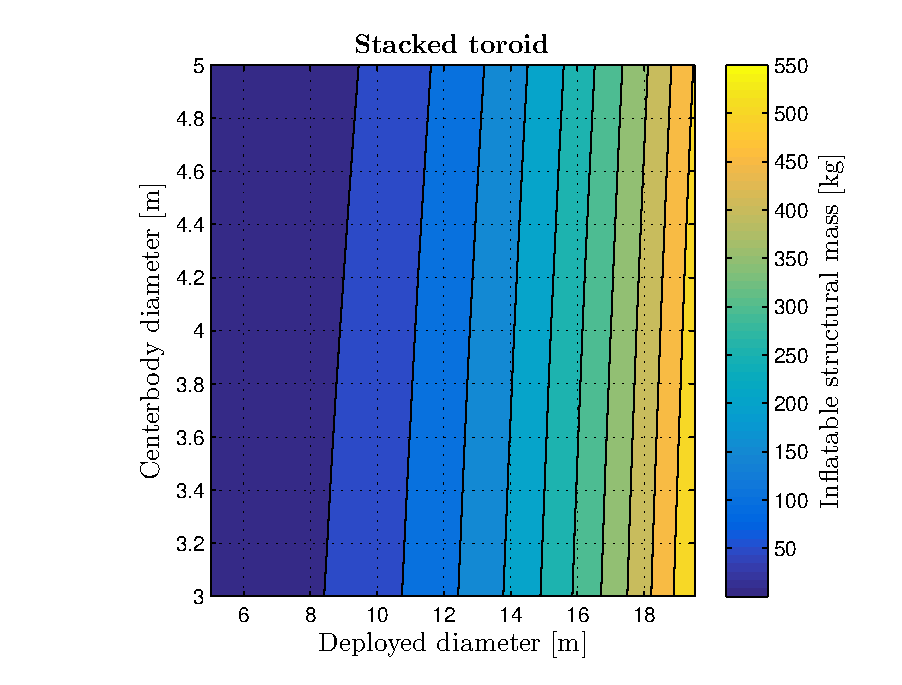
\includegraphics[width=0.96\textwidth]{./Figure/Structure/diameters_test.eps}
		\caption{Mass versus centre body and deployed diameter}
		\label{fig:diameters_strucmass}
	\end{subfigure}
	\begin{subfigure}[b]{0.49\textwidth}
		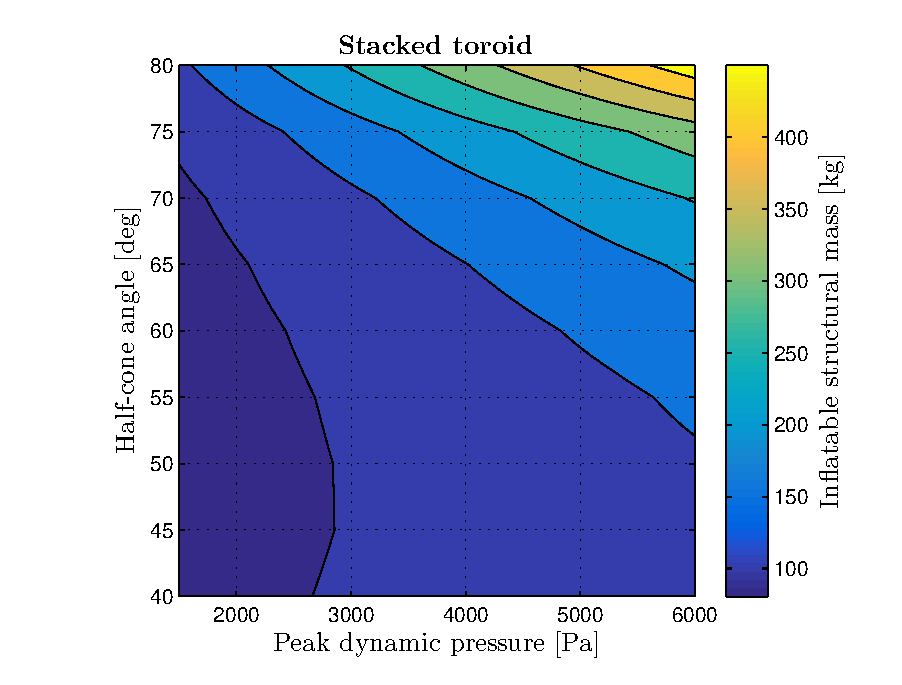
\includegraphics[width=0.96\textwidth]{./Figure/Structure/halfcone_test.eps}
		\caption{Mass versus half-cone angle and peak dynamic pressure}
		\label{fig:halfcone_strucmass}
	\end{subfigure}
	\begin{subfigure}[b]{0.49\textwidth}
		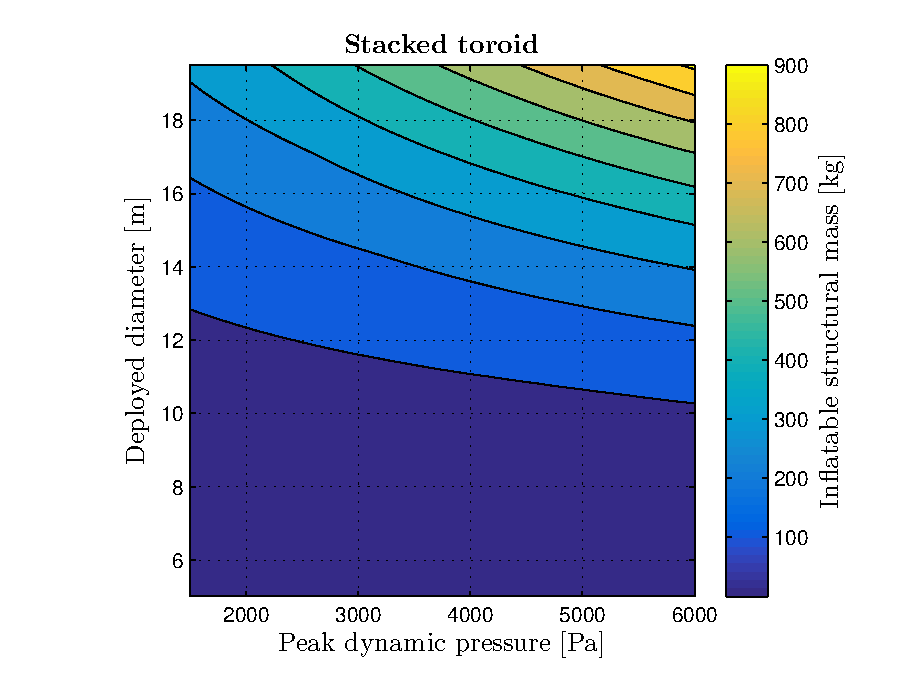
\includegraphics[width=0.96\textwidth]{./Figure/Structure/pressure_test.eps}
		\caption{Mass versus deployed diameter and peak dynamic pressure}
		\label{fig:press_strucmass}
	\end{subfigure}
	\begin{subfigure}[b]{0.49\textwidth}
		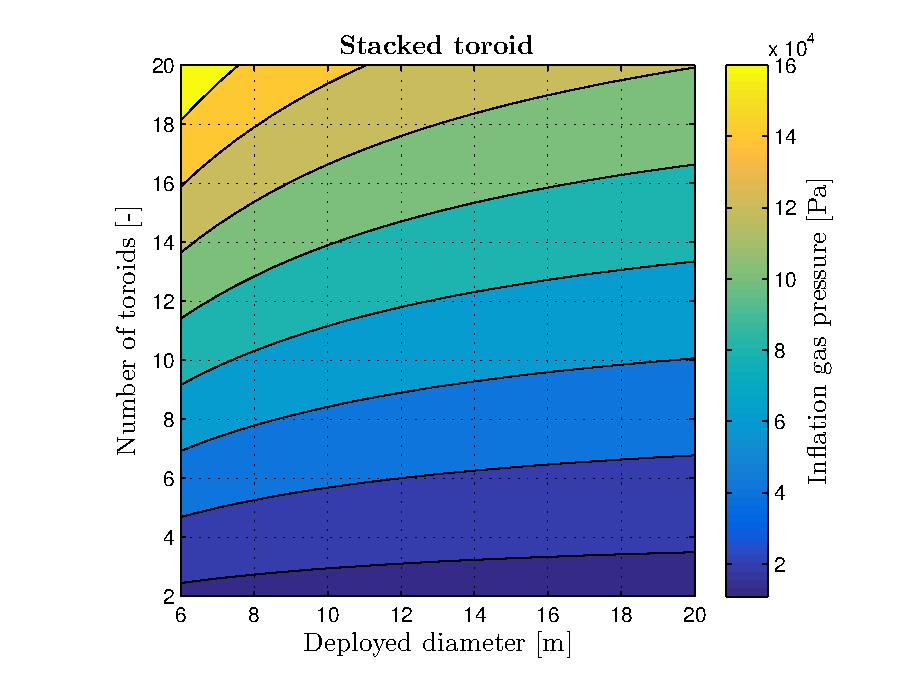
\includegraphics[width=0.96\textwidth]{./Figure/Structure/inflation_test.eps}
		\caption{Inflation pressure versus number of toroids and deployed diameter}
		\label{fig:inflpress_strucmass}
	\end{subfigure}
\caption{Inflatable structural mass and inflation pressure as a function of design parameters}
\end{figure}
Firstly, from Figure \ref{fig:diameters_strucmass} it follows that mass decreases with an increasing centre body diameter given a deployed diameter. This is due to the fact that an increasing centre body diameter increases the areal contribution of the centre body: the inflatable requires less structural mass by decreased aerodynamic loading thereof, as aerodynamic pressure works over an area. In turn, this suggests that the centre body becomes heavier, which is not the case as the centre body is typically sized for launch rather than (re-)entry loads \cite{Lindell2006}. It can therefore be concluded that maximising centre body diameter is beneficial for structural mass. 

Secondly, from Figure \ref{fig:press_strucmass} it follows that increasing dynamic pressure effects an increase in structural mass of the inflatable. This is the result of an increased aerodynamic loading and therefore structural taxation of the inflatable. To withstand this loading, extra structural mass is required. Moreover, for a given peak dynamic pressure an increase in deployed diameter effects an increase in structural mass. Primary cause hereof is the fact that pressure works over a surface area and an increase in area thereby increases the loading. This is further amplified by an increase in bending moments by the larger distance from tip to root.

From Figure \ref{fig:halfcone_strucmass} it may be observed that the half-cone angle significantly affects inflatable structural mass: in general smaller half-cone angles are preferable. Increasing half-cone angle beyond an optimum region at approximately 45 degrees strongly increases structural mass; decreasing it below this region similarly increases structural mass, but less strongly. Moreover, as aerodynamic loading is increased the optimum region shifts and smaller half-cone angles are preferable. This is due to the fact that decreasing the half-cone angle increases bending stiffness by an increased moment of inertia in the bending plane. This increased bending stiffness is further amplified by the three-dimensionality of the sphere cone and carries over to more effective use of material in bending, requiring less mass to resist the bending moment by aerodynamic loading. For a given deployed diameter, however, decreasing the half-cone angle increases the effective inflatable length. This addition of material is to be traded off against the increased bending material. At low dynamic pressures, increased bending stiffness is less warranted than at higher pressures, at which bending loads increase and bending stiffness is increasingly more warranted.

In Figure \ref{fig:inflpress_strucmass} inflation gas pressure is observed to increase for an increasing number of toroids and to decrease with an increasing deployed diameter. Both an increase in the number of toroids and a decrease in deployed diameter decrease toroid radii, effecting an increase in the working area of the inflation pressure. Due to the proportionality of the running load induced by inflation pressure via Equation \ref{eq:Pmin} with toroid radius, a larger inflation pressure is required to induce the same running load with a smaller radius. This running load is based on the consideration that the work done by inflation gas and external forces in axial direction are equal \cite{Brown2009}, independent of the number of toroids. It is similarly independent of the deployed diameter, since both inflation and aerodynamic pressure have the same working area in axial direction.
%The thickness required increases with decreasing material ultimate strength, which explains the differences in structural mass observed between different materials at low dynamic pressures. These differences carry through as loading is increased, where materials with a higher specific strength require less mass to withstand the loading. The material used in \gls{irve}-3, PBO Zylon, is observed to offer notable mass advantages over heritage aramid fibers, such as Kevlar. Mass reduction beyond this level is possible by using Technora and Spectra 2000. All materials are selected based on their operating temperature since these are required to operate in an environment with significant thermal loading. A summary of material properties is given in the Mid-Term Report \cite{Balasooriyan2015b}.
The number of toroids was observed to have no significant effect on structural mass beyond ten toroids, after which mass reductions were found to be within two percent. An increase in the number of toroids from two to ten yields significant mass advantages of up to ten percent. 



Material selection has a significant effect on flexible material mass, as illustrated by Figure \ref{fig:mat}. It can be observed that, for peak dynamic pressures below 2 [$kPa$], minimum gage thickness is leading for all selected fibres. Below this pressure, density is the leading parameter and a less dense material will perform better. Due to the significantly lower density of Spectra 2000, 970 [$kg \cdot m^{-3}$], versus that of for example PBO Zylon, 1540 [$kg \cdot m^{-3}$], Spectra 2000 offers mass advantages at low dynamic pressures. Therefore it can be concluded that for low dynamic pressures materials should be selected based on minimum gage thickness, but thickness rapidly increases as loading is increased and the minimum gage thickness is exceeded. For PBO Zylon, this occurs at a relatively high peak dynamic pressure of 3.5 [$kPa$].

For higher dynamic pressures, materials with a higher specific strength perform better in terms of structural mass. Flexible material is fully loaded in tension by the inflation pressure is required not to fail under tension, dictated by ultimate strength. To this end, a certain thickness with a corresponding mass is required. Mass performance is then directly linked to specific strength and this is confirmed by Figure \ref{fig:mat}. Aramid fibres Kevlar and Technora have the lowest specific strengths, approximately 2 [$MNm \cdot kg^{-1}$]. A notably higher specific strength of 3.44 and 3.77 [$MNm \cdot kg^{-1}$] is attained by Spectra 2000 and PBO Zylon respectively. This confirms the choice for PBO Zylon for its mass advantages over Kevlar in \gls{irve}-3 \cite{Dillman2012a}. Spectra 2000 is capable of achieving a lower mass than PBO Zylon despite its lower specific strength, due to its low density. 

Mass differences between materials remain limited, up to 30 $[kg]$ over a range of half-cone angles and diameters.

All materials have been selected based on their operating temperature since these are required to operate in an environment with significant thermal loading. As an example, Spectra 2000 fibres are not deemed suitable for their allowable temperature of 150 degrees Celsius, which would incur significant extra \acrfull{tps} mass. Dyneema would similarly be unsuitable by its temperature limit of 145 degrees Celsius\footnote{URL:\url{http://eurofibers.com/fibers/dyneema/}. Accessed: 17-06-2015} A summary of material properties is given in the Mid-Term Report \cite[p.64]{Balasooriyan2015b}. 

\begin{figure}[h]
	\centering
	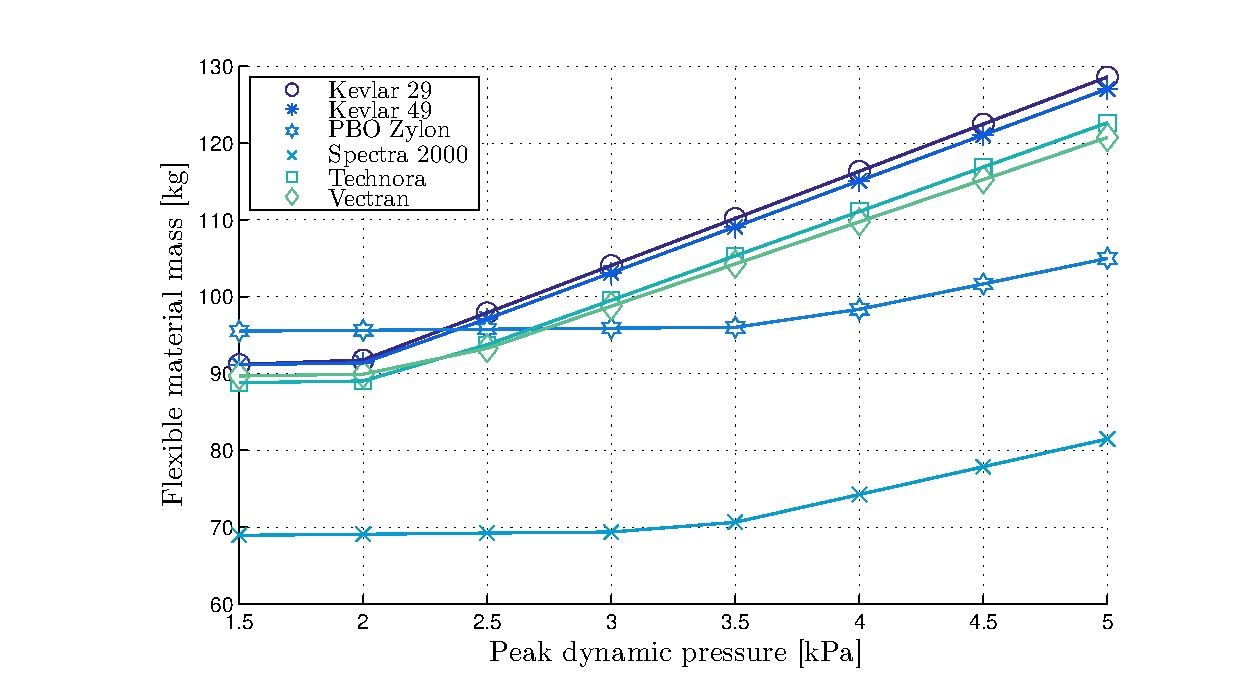
\includegraphics[width=1.0\textwidth]{./Figure/Structure/material_test2.eps}
	\caption{Flexible material structural mass estimation for different materials}
	\label{fig:mat}
\end{figure}

\paragraph{Forces}

Using the force estimation tool for the inflatable structure the sensitivity for the scaling of loads can be determined. Figure \ref{fig:forces} displays the estimated structural loads throughout the inflatable for a total of 9 toroids and a set outer diameter of 12 and 18 $[m]$. The loads as displayed in Figure \ref{fig:forces} feature solely the loads induced by aerodynamic pressure. The internal pressure loads follow separately. This sensitivity analysis is performed to evaluate the scalability of the \gls{hiad} design. Previous \gls{hiad} designs, most predominantly the \gls{irve} missions, feature smaller mission payloads and corresponding smaller diameters. Up to this point the highest diameter stacked toroid design flown is featured in the second and third \gls{irve} missions, namely an outer diameter of 2.93 $[m]$. 

\begin{figure}[h]
	\centering
	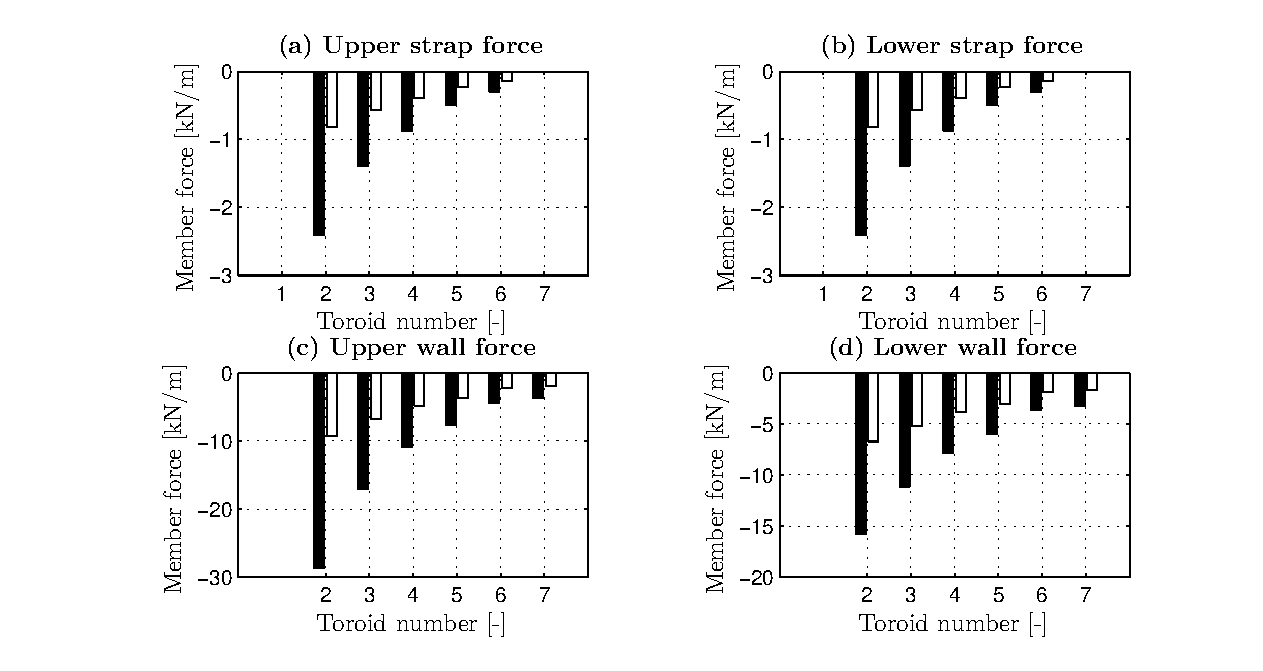
\includegraphics[width=0.9\textwidth]{./Figure/Structure/forces_nopress_test.eps}
	\caption[{Internal force estimation for dynamic pressure 3750 [$Pa$], no inflation pressure applied}]{Internal force estimation for dynamic pressure 3750 [$Pa$], no inflation pressure applied. Black bars are for a diameter of 18 [$m$]; white bars for a diameter of 12 $[m]$}
	\label{fig:forces}
\end{figure}

\begin{figure}[h]
	\centering
	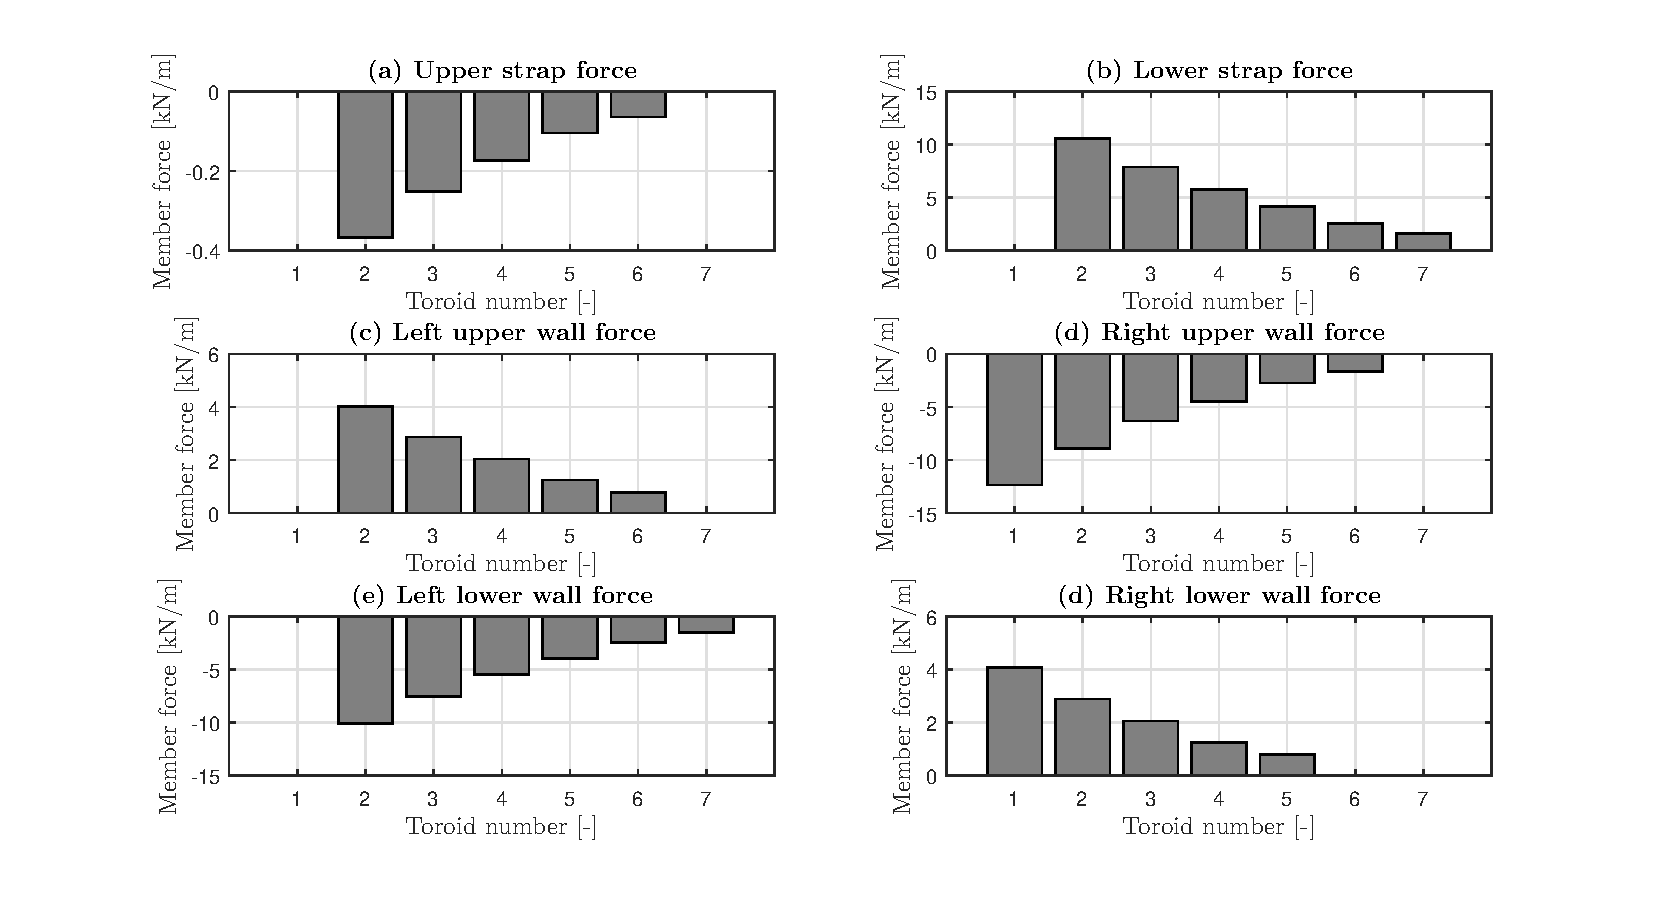
\includegraphics[width=0.9\textwidth]{./Figure/Structure/forces_test.eps}
	\caption[{Internal force estimation for dynamic pressure 3750 [$Pa$], with inflation pressure applied}]{Internal force estimation for dynamic pressure 3750 [$Pa$], with inflation pressure applied. Black bars are for a diameter of 18 [$m$]; white bars for a diameter of 12 $[m]$}
	\label{fig:forcesp}
\end{figure}

From the results of Figure \ref{fig:forces} several conclusions can be made. Most importantly it shows that scaling of the inflatable is possible. Although a load increase can be observed for increasing diameter, this follows only from the additional axial loads. The induced bending moment is not represented in Figure \ref{fig:forces} as this is carried circumferentially. This followed from the verification and validation procedures explained in more detail in Appendix \ref{sec:VandVstruc}. Moreover, loads are found to be within material capabilities.

Secondly the loads do not increase linearly over the diameter. This is the result of the scaling of the loads, to account for the decreasing circumference over which forces act. The reducing diameter causes an additional increase of the loads per unit length.

Thirdly the dynamic pressure loads of Figure \ref{fig:forces} are found to be of a similar order as the internal pressure loads induced per Equation \ref{eq:Q} at the root of the inflatable. Moving towards the tip of the inflatable these differences increase as the internal pressure loads are maintained whereas the loads induce by the dynamic pressure reduce towards the tip. This is further expanded upon in Figure \ref{fig:forcesp} in which pressure loads are included.

The final conclusion with regards to scalability of the inflatable can be made on the basis of Figure \ref{fig:forcesp}. If the internal and external pressure loads are combined a minimum required thickness can be computed on the basis of requiring the structure not to yield. This parameter is relevant as foldability of the inflatable has to be considered as well. Foldability is an important parameter as the inflatable has to be stowed away during launch and the transfer towards Mars. From this yielding criterion and a typical material such as Kevlar 49 a minimum required thickness of below 0.01 $[mm]$ is found. Since this value is rather small the thickness of the inflatable is not a consideration from a folding perspective even for large diameters.
